%!TEX root = ../thesis.tex
%*******************************************************************************
%****************************** Background Chapter *********************************
%*******************************************************************************

\chapter{Background}
\ifpdf
    \graphicspath{{Chapters/Background/Figs/}{Chapters/Background/Figs/}{Chapters/Background/Figs/}}
\else
    \graphicspath{{Chapters/Background/Figs/}{Chapters/Background/Figs/}}
\fi
To build the foundation of our approach, we present the usage of crowdsourcing in software development (see section \ref{background:section:crowdsourcing}), UI Prototyping (see section \ref{background:section:uiprototyping}), Low and No code (see section \ref{background:section:lowcode}), Model Based Software Engineering (MBSE) (see section \ref{background:section:mbse}), Task Based Usability Testing (see section \ref{background:section:task}), and Experimental Product Design and define Design Principles (DP) (see section \ref{background:section:experimentproduct}).

%********************************** % Crowdsourcing of Software Products **************************************
\section{Crowdsourcing of Software Products}
\label{background:section:crowdsourcing}
Iterative feedback from potential customers can help improve the development of software products \cite{article:lean:eric}.
To do that, we can use crowdsourcing.
Crowdsourcing refers to outsourcing value-creating activities from a company by an open call to a large, undefined group of users to get feedback \cite{article:crowdsourcing:leimeister}.
The word crowdsourcing is a combination of crowd and outsourcing.
Crowdsourcing often involves less specialized and more generalized groups of participants than outsourcing \cite{article:crowdsourcing:estelles}.
Some advantages of crowdsourcing include lowered costs, improved speed, quality, flexibility, and scalability \cite{article:crowdsourcing:prpic}.
Researchers have used crowdsourcing in many research approaches, including \textit{crowd testing, crowd funding, crowd ideation, crowd logistic, crowd production, crowd promotion,} and \textit{crowd support} over the last few years \cite{article:crowdsourcing:durward}.
In our approach to finding a solution, we focus more on crowd-testing and crowd-ideation.

\paragraph{Crowd Testing:}
The companies use crowd-testing to evaluate different running software products with the users.
A growing trend in software testing is crowd testing, which utilizes the benefits, effectiveness, and efficiency of crowdsourcing and cloud platforms \cite{article:crowdsourcing:latoza}.
Crowd testing is considered when the software is more user-centric: i.e., software with a broad user base whose success is evaluated by user input.
CrowdStudy \cite{article:crowdsourcing:nebeling} is a method that enables developers to assess the usability of their web interfaces using crowd workers from Amazon Mechanical Turk\footnote{Amazon Mechanical Turk: \url{https://www.mturk.com}}.
CrowdCrit \cite{article:crowdsourcing:luther} is another tool that uses Amazon Mechanical Turk to support designers in validating created posters in the form of uploaded images.
Similarly, \textit{Interactive event-flow graphs} and \textit{GUI-level (Graphical User Interface) guidance} \cite{article:crowdsourcing:chen} are the two techniques to increase crowd testers' coverage for GUI using crowd-testing.

\paragraph{Crowd Ideation:}
Design can be infused with creativity by online crowds, but using traditional strategies to harness them, such as large-scale ideation platforms, requires organization and time \cite{article:crowdsourcing:andolina}.
Hence, crowd ideation is used to build new and improved versions of existing software product ideas with the consumers.
Under manipulations of task complexity, idea representation, and procedural guidance, Shixuan Fu et al. \cite{article:crowdsourcing:fu} examine how cognitive load is altered during idea generation and convergence with crowds.
ERICA \cite{article:crowdsourcing:erica} is a tool that uses expert knowledge to validate diverse crowd answers.
Crowdboard \cite{article:crowdsourcing:andolina} is a tool used to engage crowds in real-time brainstorming, concept mapping, and other design processes at an early stage of the design process.
There were, however, no approaches that directly addressed prototype application areas.

%********************************** % UI Prototyping **************************************
\section{UI Prototyping}
\label{background:section:uiprototyping}
User Interface prototyping is an evaluation and testing technique according to User-Centred Design (UCD) methodology since the 1990s \cite{article:prototyping:preece}. 
The evaluation of prototypes by users is a fundamental part of all iterative approaches for IT project management, especially agile methodologies \cite{article:prototyping:schwaber}.
And to build an exemplary user interface, iterative refinement must be used: develop a preliminary version of the user interface, test it with people, and make as many revisions as possible \cite{article:prototyping:gould}.
Therefore, designing UI prototypes enables designers and stakeholders to communicate more effectively.
An interactive prototype helps visualize design concepts and communicate new requirements and expectations about a prospective system.
Iterative design requires multiple updates to the design's execution.
Since developing and updating the entire software system is complex and expensive, prototyping is a crucial technique \cite{article:prototyping:szekely}.
Simultaneously, software prototypes might exclude many requirements, making the software more accessible, smaller, and less expensive to construct and change \cite{article:prototyping:szekely}. 
Similarly, usability testing to validate user requirements and prototype functionality is part of the evaluation process for UI prototypes.
When prototyping is used, there is usually more contact between the designers and users, resulting in fewer usability flaws and corrections at the end of development.

Jim Rudd et al. \cite{article:prototyping:highlowfidelity} have compared high and low-fidelity prototyping, explaining the advantages and disadvantages.
\textit{Low-fidelity} prototypes are usually limited function, with little interaction prototyping effort. They mainly focus on explaining concepts, design alternatives, and screen layouts. 
Storyboard presentations, cards, and proof of concept prototypes come under this category.
These prototypes emphasize communicating, educating, and informing rather than training, testing, and codification.
The advantages of low-fidelity prototypes are rapid development, lower development cost, addressing issues, and usefulness for a proof-of-concept.
Similarly, the disadvantages include limited error checking, difficulty with usability testing, navigation, flow limitation, etc.
Contrary to low-fidelity prototypes, \textit{High-fidelity} prototypes have full functionality and focus on flow, and the user models of the system \cite{article:prototyping:exploratory}.
The users can operate these prototypes, and the developers can collect information from the users through measurements. 
Other advantages of high-fidelity prototypes are that they are user-driven, used for navigation and tests, and can also be served as a marketing tool for attracting potential customers \cite{article:prototyping:highlowfidelity}.

% \begin{figure}[htbp!]
% \centering    
% 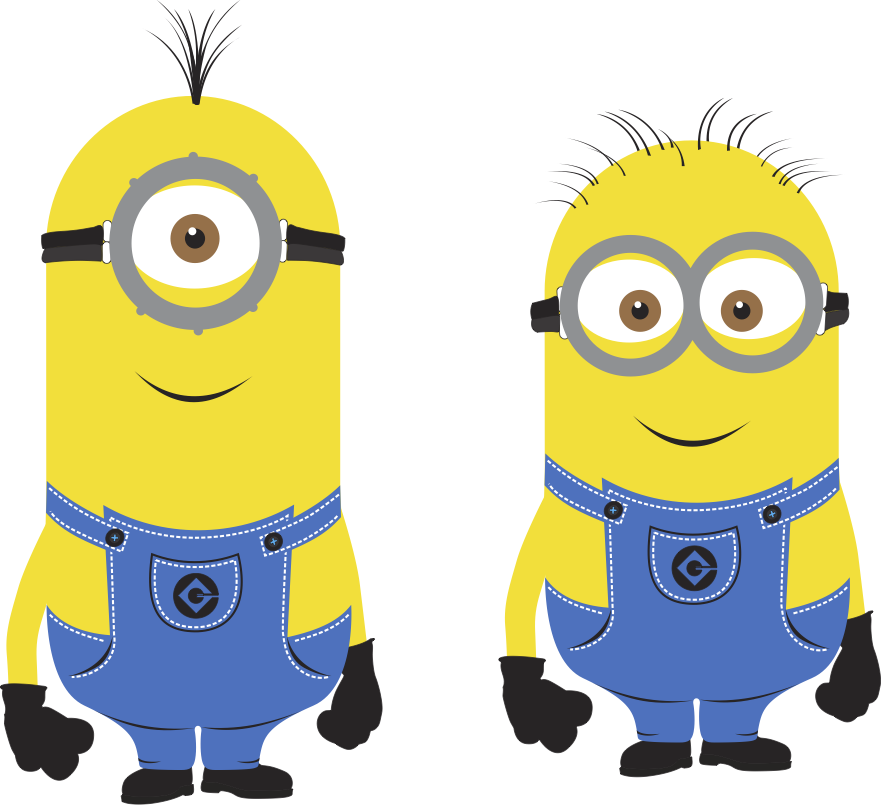
\includegraphics[width=1.0\textwidth]{minion.png}
% \caption[Minion]{This is just a long figure caption for the minion in Despicable Me from Pixar}
% \label{fig:minion}
% \end{figure}

%********************************** % Low code **************************************
\section{Low Code / No Code Development Platform}
\label{background:section:lowcode}
Low Code is a technique used by developers to help non-developers design and develop software applications using a \textit{Graphical User Interface} (GUI) supported by a \textit{Low Code Development Platform} (LCDP).
Similarly, there is another technique called No code supported by the \textit{No Code Development Platform} (NCDP) \cite{article:nocode:miller}.
Unlike low code, no-code platforms require no programming skills because they offer some prebuild templates for building the apps.
Using the visual user interface and ready-made automatic tools on these application development platforms, it is feasible to create apps relatively quickly. 

Drag-and-drop technologies offered by no-code development platforms allow companies and non-developers to create software quickly without writing code.
Due to its simplicity, flexibility and low cost, companies have started using this platform to meet the high demands of software development and digitalization.
Low code is a software development method that uses less human coding to enable users to construct and manage programs efficiently \cite{article:nocode:sahina}.
Additionally, it lowers the expenses associated with initial installation, training, distribution, and maintenance \cite{article:nocode:sanchi}.

\begin{itemize}
  \item[] \textbf{Some features that make the LCDP or NCDP favorable for development}
  \item \textbf{Transparency:} \cite{article:nocode:sahina} The platforms are accessible to everyone.
  \item \textbf{Scalable:} \cite{article:nocode:ihirwe, article:nocode:sahina} These platforms are built to make the software scalable.
  \item \textbf{Flexible and Model-driven development:} \cite{paper:lowcode:cabot} Low code has become famous among model-driven development.
  \item \textbf{Easy deployment:} \cite{article:nocode:ihirwe} This feature ensures that the artifacts are created and the platform is ready to deploy.
  \item \textbf{User Interface:} \cite{article:nocode:sahina} LCDP ensures to have a GUI useful for the non-developers.
\end{itemize}

Additionally, a variety of options are provided for developers with little programming experience, those with coding expertise and seasoned programmers who wish to expand the functionality of the current design \cite{article:nocode:sahina}.

%********************************** % Model-Based Software Engineering **************************************
\section{Model-based Software Engineering}
\label{background:section:mbse}
Model-based Software Engineering (MBSE) refers to maintaining and developing software while reusing existing code.
Similarly, Model-driven software engineering (MDSE) is the term used to cover various techniques for creating software using codified models.
The development of domain-specific languages (DSLs) is becoming essential in language engineering due to the growth in model-driven engineering (MDE) \cite{article:mbse:cuadrado}.
MDSE has become an integral part of developing User interfaces, and they have been named Model-driven User Interfaces (MUIs).
Based on that, adaptive model-driven user interface development systems are developed \cite{article:mbse:akiki}.
In this research, the authors defined twenty properties challenges for the Model-driven User interface and compared some tools that implement these properties.

Companies use different modeling languages to codify the UIs.
Cameleon \cite{article:cameleon:balme} is a framework that divides the UI into several elements to maximize the parts' reusability in various user, platform, and environment situations.
A platform-independent abstract UI, a platform-dependent concrete UI, and a device-dependent final UI are the layers the framework offers to accomplish this.
A standardized modeling language for software product content, abstract UI models, user interactions, and control behavior is Interaction Flow Modeling Language (IFML) \cite{article:ifml:piero}.
As a result, IFML relies on the platform-independent display of the UI that can be utilized on several platforms and devices.

However, these modeling languages do not emphasize offering visual notations to aid non-developers in creating such interfaces. 
A recent method \cite{article:mbse:bexiga} illustrates how to use low-code approaches to close the gap between designers and developers.

%********************************** % Task-based Usability Testing **************************************
\section{Task-based Usability Testing}
\label{background:section:task}
The main focus of usability testing is that seeing someone use an interface is the best approach to determine what functions well and what doesn't. 
Assigning tasks to the accurate number of participants can help determine the quality of the UI and the problems faced by the users. 
Overall, the UI design can be improved using the participants' feedback. 
Task-based usability testing is one way to determine the software's overall usability \cite{article:usability:doesburg} by measuring the percentage of the tasks the users complete.
To observe the participants, they need to be assigned some ``activities'' or \textit{tasks}. 
These tasks need to be some scenarios, not just "\textit{do something}", because it sets the users a stage for \textit{why} they would perform the tasks. 
To get qualitative feedback from the participants, in \cite{misc:usability:tasks}, the authors provide \textit{three good practices} and task-writing tips for designing better task scenarios.
\textit{(1) Make the Task Realistic}.
So, the participants should be able to execute the tasks which could be completed efficiently and with the freedom to make their own choices.
\textit{(2) Make the Task Actionable}.
Here, the participants should be told what they need to do rather than how they would do it.
\textit{(3) Avoid Giving Clues and Describing the Steps}.
The participants should expose the navigation and some features on their own, giving accurate feedback about the interface.
The task scenario example\footnote{Task based usability: \url{https://www.nngroup.com/articles/task-scenarios-usability-testing/}} below sets a target for the participants to locate a movie from our \textit{Videostreamer} app.
\begin{itemize}
  \item[] \textbf{Good and bad example of a task scenario}
  \item \textbf{User goal:} Find a movie. 
  \item \textbf{Bad task scenario:} You should watch a movie on Sunday afternoon. Go to\\ \textit{www.videostreamer.com}, navigate to the Movies page, and find the movie as per the schedule.
  \item \textbf{Good task scenario:} Use \textit{www.videostreamer.com} to find a movie that fits your interest that you'd be interested in watching on Sunday afternoon. 
\end{itemize}
In this example, the \textit{bad} task scenario gives detailed information about the navigation, violating the third tip.

%********************************** % Experimentation **************************************
\section{Experimentation}
\label{background:section:experimentproduct}
Experimental Product Design (EPD) has become integral to optimizing UI and \textit{User Experience (UX)}.
Experimentation helps product teams test out ideas early in the process with real-world consumers rather than settling on a single solution and executing it in the final phase \cite{misc:CE:miklos}.
In this section, we discuss the role that experimentation plays in the software development process and how designers can ``prototype with real data'' to improve the usability of the UI.

\paragraph{Continuous Experimentation:} 
Continuous experimentation (CE) primarily aims to get users' feedback on the software product's evolution.
CE generally uses A/B/n testing in a primary case of comparing two variants, A and B, which are controlled and test variables in an experiment.
With CE, developers make evidence-based decisions to direct the progress of their software by continuously measuring the results of multiple variants performed in an experimental context with actual users \cite{article:CE:ros}.
CE is an extension to the introduction of continuous integration and deployment, and all are summarized as constant software engineering \cite{article:CE:fitzgerald}.

% \clearpage

% \begin{landscape}

% \section{Landscape}
% I can cite Wall-E (see Fig.~\ref{fig:WallE}) and Minions in despicable me (Fig.~\ref{fig:Minnion}) or I can cite the whole figure as Fig.~\ref{fig:animations}


% \begin{figure}
%   \centering
%   \begin{subfigure}[b]{0.3\textwidth}
%     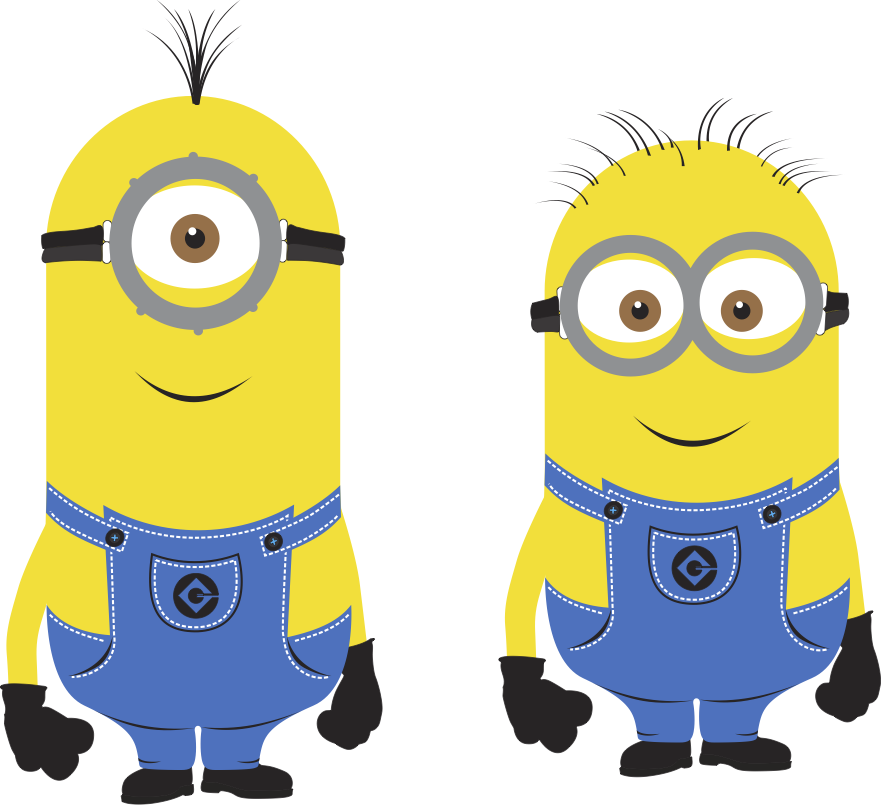
\includegraphics[width=\textwidth]{minion.png}
%     \caption{Tom and Jerry}
%     \label{fig:TomJerry}   
%   \end{subfigure}             
%   \begin{subfigure}[b]{0.3\textwidth}
%     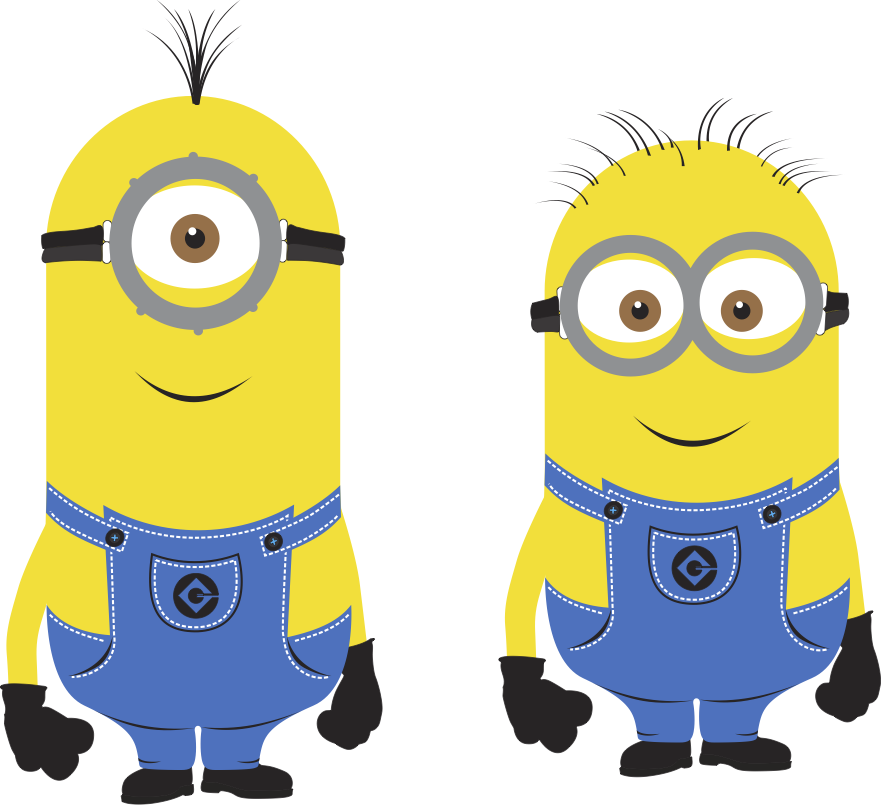
\includegraphics[width=\textwidth]{minion.png}
%     \caption{Wall-E}
%     \label{fig:WallE}
%   \end{subfigure}             
%   \begin{subfigure}[b]{0.3\textwidth}
%     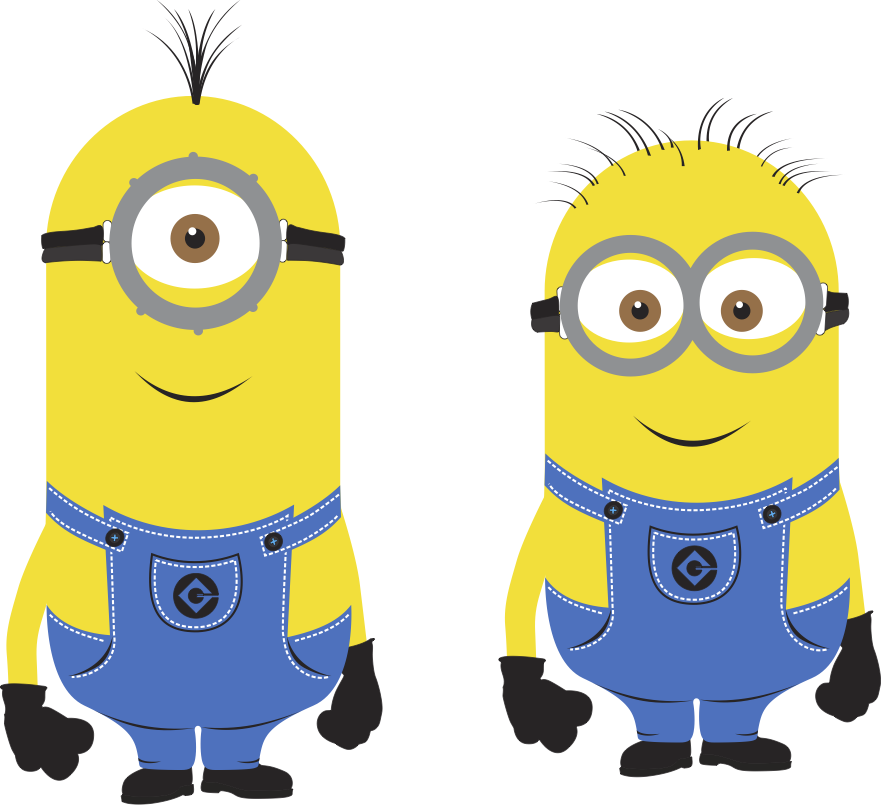
\includegraphics[width=\textwidth]{minion}
%     \caption{Minions}
%     \label{fig:Minnion}
%   \end{subfigure}
%   \caption{Best Animations}
%   \label{fig:animations}
% \end{figure}

% \end{landscape}
